\documentclass{article}
\usepackage{amsmath}
\usepackage{amssymb}
\usepackage[a4paper, top=25mm, bottom=25mm, left=25mm, right=25mm]{geometry}
\usepackage{pgfplots}
\usepackage{cancel}
\usepackage{mathtools}
\pgfplotsset{compat=1.18}
\usepgfplotslibrary{polar}
\usepgfplotslibrary{fillbetween}

\begin{document}
\pagestyle{empty}
\large

\begin{center}
2023-2024 Spring \\MAT124 Makeup\\(27/06/2024)
\end{center}

\noindent 1. Find the maximum and minimum values of $f(x,y,z)=x-y+z$ on the sphere $x^2+y^2+z^2=100$.

\hfill

\noindent 2. Sketch the region and reverse the order of the double integral

\[\int_0^{\bcancel4\:3}\int_{y/3}^{\sqrt{4-y}}dx\,dy\]

\hfill

\noindent 3. Using a polar double integral, find the volume of the sphere with radius $4$.

\hfill

\noindent 4. Find the surface area of the portion of the paraboloid $z=x^2+y^2$ that lies in the cylinder $x^2+y^2=1$.

\hfill

\noindent 5. Using the change of variables, evaluate the area of the ellipse $\displaystyle\frac{x^2}{16}+\frac{y^2}{25}=1$.

\hfill

\noindent 6. Let $R$ be the solid region bounded below by the cone $z=\sqrt{3x^2+3y^2}$ and above by the sphere $x^2+y^2+z^2=9$. Let

\[\mathrm{I}=\iiint_R(x^2+y^2)\,dV.\]

\hfill

\noindent (i) Express (but do not evaluate) $\mathrm{I}$ as a triple integral in spherical coordinates.

\hfill

\noindent (ii) Express (but do not evaluate) $\mathrm{I}$ as a triple integral in cylindrical coordinates.

\newpage

\begin{center}
2023-2024 Spring Makeup (27/06/2024) Solutions\\
(Last update: 8/5/25 (5th of August) 12:51 AM)
\end{center}

\noindent 1. Let $g(x,y,z)=x^2+y^2+z^2-100$ for the constraint. Solve the system of equations below.

\[
\left.
\begin{array}{l}
\displaystyle\nabla f=\lambda\nabla g \\
\displaystyle g(x,y,z)=0
\end{array}
\right\}\quad
\begin{array}{c}
\nabla f=\left\langle1,-1,1\right\rangle=\lambda\left\langle2x,2y,2z\right\rangle=\lambda\nabla g
\end{array}
\]

\[1-2\lambda x=0\implies x=\frac1{2\lambda}\]
\[-1-2\lambda y=0\implies y=-\frac1{2\lambda}\]
\[1-2\lambda z=0\implies z=\frac1{2\lambda}\]

\hfill

\noindent Use the constraint to find the values of $x,\:y,\:z$.

\[x^2+y^2+z^2-100=0\implies\left(\frac1{2\lambda}\right)^2+\left(-\frac1{2\lambda}\right)^2+\left(\frac1{2\lambda}\right)^2=\frac3{4\lambda^2}=100\implies\lambda=\pm\frac{\sqrt3}{20}\]

\[x=\frac1{2\lambda}=\pm\frac{10\sqrt3}3,\quad y=-\frac1{2\lambda}=\pm\frac{10\sqrt3}3,\quad z=\frac1{2\lambda}=\pm\frac{10\sqrt3}3\]

\hfill

\noindent To find the maximum and minimum values of $f$, use the points $\left(\frac{10\sqrt3}3,-\frac{10\sqrt3}3,\frac{10\sqrt3}3\right)$ and $\left(-\frac{10\sqrt3}3,\frac{10\sqrt3}3,-\frac{10\sqrt3}3\right)$, respectively.

\hfill

\[
\boxed{\begin{array}{c}
\displaystyle f_{\text{max}}=\frac{10\sqrt3}3-\left(-\frac{10\sqrt3}3\right)+\frac{10\sqrt3}3=10\sqrt3\\
\displaystyle f_{\text{min}}=-\frac{10\sqrt3}3-\frac{10\sqrt3}3-\frac{10\sqrt3}3=-10\sqrt3\end{array}}
\]

\hfill

\noindent 2. \textbf{Remark}: It is counterintuitive that the area of the region is negative for $y>3$. Therefore, let's assume that the upper bound for $y$ is $3$ rather than the value stated in the original question. The lecturer might have made a typo.

\begin{center}
\begin{minipage}{0.45\textwidth}
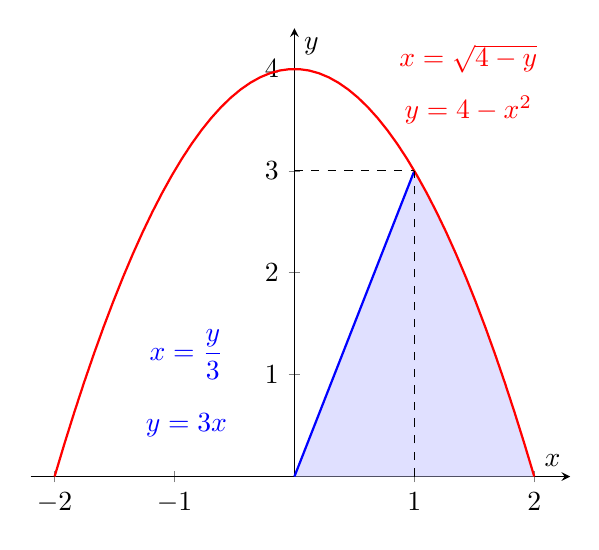
\begin{tikzpicture}
  \begin{axis}[
      axis lines=center,
      xlabel={$x$},
      ylabel={$y$},
      xmin=-2.2, xmax=2.3,
      ymin=0, ymax=4.4,
      samples=50,
      clip=true,
      scale=1,
    ]

    \addplot [thick, blue, domain=0:1] {3*x};
    \addplot [thick, red, domain=-2:2] {4-x^2};
    \addplot [draw=none, name path=upper, domain=0:2] {min(3*x,4-x^2)};
    \addplot [draw=none, name path=lower, domain=0:2] {0};

    \addplot [
      blue!20,
      fill opacity=0.6,
    ] fill between[of=lower and upper, soft clip={domain=0:2}];

    \node[blue] at (axis cs:-0.9,1.2) {$\displaystyle x=\frac y3$};
    \node[blue] at (axis cs:-0.9,0.5) {$y=3x$};

    \node[red] at (axis cs:1.45,4.1) {$x=\sqrt{4-y}$};
    \node[red] at (axis cs:1.45,3.6) {$y=4-x^2$};

    \draw[dashed] (0,3) -- (1,3);
    \draw[dashed] (1,0) -- (1,3);
  \end{axis}
\end{tikzpicture}
\end{minipage}
\begin{minipage}{0.45\textwidth}
\[\boxed{\int_0^1\int_0^{3x}dy\,dx+\int_1^2\int_0^{4-x^2}dy\,dx}\]
\end{minipage}
\end{center}

\newpage

\noindent 3. The equation of this sphere is $x^2+y^2+z^2=16$. Solve for $z$ to find the bounds of $z$.

\[z_{\text{lower}}=-\sqrt{16-x^2-y^2},\quad z_{\text{upper}}=\sqrt{16-x^2-y^2}\]

\hfill

\noindent If we project the sphere onto the $xy$-plane, we will notice that the domain is $x^2+y^2\leq16$. Use the transformation for polar coordinates.

\[
\begin{array}{c}
x=r\cos\theta\\
y=r\sin\theta\\
x^2+y^2=r^2\\
dA=r\,dr\,d\theta
\end{array}\quad\rightarrow\quad
\begin{array}{c}
z=\sqrt{16-x^2-y^2}\implies z=\sqrt{16-r^2}\\[0.2cm]
z=-\sqrt{16-x^2-y^2}\implies z=-\sqrt{16-r^2}\\[0.2cm]
x^2+y^2\leq16\implies r^2\leq 16\implies 0\leq r\leq 4,\quad \displaystyle0\leq\theta\leq2\pi
\end{array} 
\]

\begin{align*}\mathrm{I}&=\int_0^{2\pi}\int_0^4\left[\sqrt{16-r^2}-\left(\sqrt{16-r^2}\right)\right]\,r\,dr\,d\theta=2\int_0^{2\pi}\int_0^4r\sqrt{16-r^2}\,dr\,d\theta\\\\&=2\int_0^{2\pi}\left[-\frac13\left(16-r^2\right)^{3/2}\right]_{r=0}^{r=4}\,d\theta=\frac23\int_0^{2\pi}\left[0-\left(-64\right)\right]\,d\theta=\frac{128}3\int_0^{2\pi}d\theta=\boxed{\frac{256\pi}3}\end{align*}

\hfill

\noindent 4. The domain is $x^2+y^2\leq1$. Using the double integral below, we find the surface area.

\begin{align*}
\text{Surface area}&=\iint_D\sqrt{1+\left(\frac{\partial z}{\partial x}\right)^2 +\left(\frac{\partial z}{\partial y}\right)^2}\,dA=\int_{-1}^1\int_{-\sqrt{1-x^2}}^{\sqrt{1-x^2}}\sqrt{1+\left(2x\right)^2 +\left(2y\right)^2}\,dy\,dx\\\\&=\int_{-1}^1\int_{-\sqrt{1-x^2}}^{\sqrt{1-x^2}}\sqrt{1+4x^2+4y^2}\,dy\,dx
\end{align*}

\hfill

\noindent If we switch to polar coordinates, we can easily evaluate the integral.

\begin{align*}\text{Surface area}&=\int_0^{2\pi}\int_0^1\sqrt{1+4r^2}\,r\,dr\,d\theta=\frac1{12}\int_0^{2\pi}\left[\left(1+4r^2\right)^{3/2}\right]_{r=0}^{r=1}\,d\theta\\\\&=\frac1{12}\int_0^{2\pi}\left(5\sqrt5-1\right)\,d\theta=\boxed{\frac\pi6\left(5\sqrt5-1\right)}\end{align*}

\hfill

\noindent 5. Let $x=4r\cos\theta,\:y=5r\sin\theta$.

\[\frac{x^2}{16}+\frac{y^2}{25}=1\implies\frac{(4r\cos\theta)^2}{16}+\frac{(5r\sin\theta)^2}{25}=1\implies r^2\left(\sin^2\theta+\cos^2\theta\right)=1\]
\[r^2=1\implies r=1\quad\quad0\leq\theta\leq2\pi\]

\newpage

\noindent Calculate the Jacobian determinant.

\hfill

\[
\left|\frac{\partial(x,y)}{\partial(r,\theta)}\right|=\left|\begin{array}{cc}
\displaystyle\frac{\partial x}{\partial r}&\displaystyle\frac{\partial x}{\partial\theta}\\[1em]
\displaystyle\frac{\partial y}{\partial r}&\displaystyle\frac{\partial y}{\partial\theta}
\end{array}\right|=\left|\begin{array}{cc}
4\cos\theta&-4r\sin\theta\\
5\sin\theta&5r\cos\theta
\end{array}\right|=20r\cos^2\theta-\left(-20r\sin^2\theta\right)=20r
\]

\hfill

\noindent Then we have the integral

\begin{align*}\int_0^{2\pi}\int_0^1\left|\frac{\partial(x,y)}{\partial(r,\theta)}\right|\,dr\,d\theta&=\int_0^{2\pi}\int_0^120r\,dr\,d\theta=20\int_0^{2\pi}\left[\frac12r^2\right]_{r=0}^{r=1}d\theta=10\int_0^{2\pi}d\theta=\boxed{20\pi}\end{align*}

\noindent 6.

\hfill

\noindent (i) For spherical coordinates, we have

\[
\begin{array}{c}
z=\rho\cos\phi\\
r=\rho\sin\phi\\
x^2+y^2=r^2\\
x^2+y^2+z^2=\rho^2\\
dV=\rho^2\sin\phi\,d\rho\,d\phi\,d\theta
\end{array}\quad\rightarrow\quad
\begin{array}{c}
\displaystyle z=\sqrt{3x^2+3y^2}\implies\rho\cos\phi=\sqrt3\rho\sin\phi\implies\phi=\frac\pi6\\[0.2cm]
x^2+y^2=r^2=\rho^2\sin^2\phi\\[0.1cm]
x^2+y^2+z^2=9\implies\rho^2=9\implies\rho=3\\[0.1cm]
0\leq\theta\leq2\pi
\end{array}
\]

\hfill

\noindent The integral in spherical coordinates can be expressed as follows.

\[\boxed{\mathrm{I}=\int_0^{2\pi}\int_0^{\pi/6}\int_{0}^3\rho^2\sin^2\phi\cdot\rho^2\sin\phi\,d\rho\,d\phi\,d\theta=\int_0^{2\pi}\int_0^{\pi/6}\int_{0}^3\rho^4\sin^3\phi\,d\rho\,d\phi\,d\theta}\]

\hfill

\noindent (ii) For cylindrical coordinates, we have

\[
\begin{array}{c}
z=z\\
r^2=x^2+y^2\\
dV=r\,dz\,dr\,d\theta
\end{array}\quad\rightarrow\quad
\begin{array}{c}
z=\sqrt{3x^2+3y^2}\implies z=r\sqrt3\\[0.1cm]
x^2+y^2=r^2\\[0.1cm]
x^2+y^2+z^2=9\implies z=\sqrt{9-r^2}\\[0.1cm]
0\leq\theta\leq2\pi
\end{array}
\]

\hfill

\noindent Find where the curves intersect to find the upper limit of $r$.

\[r\sqrt3=\sqrt{9-r^2}\implies3r^2=9-r^2\implies r^2=\frac94\implies r=\frac32\]

\hfill

\noindent The integral in cylindrical coordinates can be expressed as follows.

\[\boxed{\mathrm{I}=\int_0^{2\pi}\int_0^{3/2}\int_{r\sqrt3}^{\sqrt{9-r^2}}r^2\cdot r\,dz\,dr\,d\theta=\int_0^{2\pi}\int_0^{3/2}\int_{r\sqrt3}^{\sqrt{9-r^2}}r^3\,dz\,dr\,d\theta}\]

\end{document}